\documentclass[conference]{IEEEtran}
\IEEEoverridecommandlockouts
\usepackage{cite}
\usepackage{amsmath,amssymb,amsfonts}
\usepackage{graphicx}
\graphicspath{{figures/}{paper/figures/}}
\usepackage{textcomp}
\usepackage{xcolor}
\usepackage{booktabs}
\usepackage{url}

% Rough-draft markers. Delete every \todo before submission.
\newcommand{\todo}[1]{\textcolor{red}{[TODO: #1]}}

\begin{document}

\title{From Paper to Pipeline: An Agentic Loop for Porting and\\
Iso-Budget Tuning of Published Microarchitecture Features}

\author{\IEEEauthorblockN{Evan Lai}
\IEEEauthorblockA{\textit{Stanford University}\\
evanxlai@stanford.edu}
\and
\IEEEauthorblockN{Jan Strzeszynski}
\IEEEauthorblockA{\textit{\todo{affiliation}}\\
\todo{email}}
}

\maketitle

\begin{abstract}
Evaluating a feature from a recent paper on one's own infrastructure is slow
for two reasons. A reference implementation may not exist, or targets a
different simulator and baseline. And a published parameterization was tuned
for a different host, so an untuned port measures the port rather than the
idea. We present an adopt-a-paper loop, built on the CHIA agentic framework,
that takes a host design, a paper, and success criteria. It distills the paper
into a structured feature spec, plans the port against the real host, has a
coding agent integrate the feature behind a deterministic verify gate, and then
tunes the feature jointly with the host's own sizing under a storage
constraint. Only the tuned configuration is compared against the baseline. We
demonstrate the loop by porting the register-value statistical-corrector
component of RUNLTS, the CBP2025 winner, into the CBP2025 kit's TAGE-SC-L and
tuning it at 64 KiB. The gate caught every broken port we observed, including a
port that passed all correctness tests but made cycles-on-wrong-path 43 percent
worse, and agents escalated questions outside their authority rather than
weakening tests. The tuned verdict is small and fragile: across three searches,
the tuned candidate changed held-out MPKI by between 0.34 percent better and
0.76 percent worse than the unmodified host. We report what the loop got wrong
along the way, since most of what we learned came from those failures.
\end{abstract}

\begin{IEEEkeywords}
branch prediction, design-space exploration, LLM agents, simulation,
reproducibility
\end{IEEEkeywords}

%----------------------------------------------------------------------
\section{Introduction}

A computer architect who wants to know whether a newly published mechanism
helps their design has to do two expensive things. First, they must implement
it on their own simulator, often from the paper alone. Second, they must tune
it. A paper's parameters were chosen for the authors' host under the authors'
budget. Dropping those parameters into a different host and comparing against
that host's baseline mostly measures how well the parameters happen to
transfer. A fair comparison holds a resource budget fixed and lets both the
feature and the host re-balance within it.

We automate both halves with an \emph{adopt-a-paper} loop. Its inputs are (i) a
target design $A$, (ii) a feature $F$ described by a paper, with a reference
artifact as an optional input, and (iii) success criteria. The loop plans how
$F$ goes into $A$, integrates it, verifies it, and then runs a design-space
exploration (DSE) over $F$'s parameters and $A$'s sizing under a constraint
set. The verdict is the tuned configuration against the baseline.

Two rules shape the design:
\begin{itemize}
\item \textbf{Agents never self-report success.} Every pass/fail decision is a
programmatic edge in plain code. Agents reach the host only through tools
(shell, build, run, stats), and a gate measures the result.
\item \textbf{Only the DSE stage knows about resource constraints.} Every
earlier stage is about implementing the feature correctly. A storage budget
enters as one allowance in stage 4's constraint set.
\end{itemize}

Our demonstration ports sR, the register-value component of RUNLTS~\cite{runlts},
into the CBP2025 kit's TAGE-SC-L~\cite{cbp2025kit,tagescl}. RUNLTS won CBP2025,
and its paper describes sR in enough detail to implement but gives no
stand-alone number for sR's gain.

Our contributions are:
\begin{enumerate}
\item A staged loop (distill, spec review, plan, integrate, tune, promote) with
typed JSON contracts between stages and a six-condition deterministic gate
(Section~\ref{sec:loop}).
\item An \emph{escalation} channel: an integrating agent that believes a frozen
value in its plan is wrong names it, and the job re-runs planning with that
question attached, rather than letting the agent edit its own success criteria.
\item Constraint-aware tuning in which the host's own sizing defines are
knobs, storage is recomputed from each candidate's header before it is built,
and a preflight proves every storage-costing knob actually changes the binary.
\item An end-to-end run on a GCP cluster, including the negative results and a
catalogue of the loop failures that produced them (Section~\ref{sec:results}).
\end{enumerate}

%----------------------------------------------------------------------
\section{Background}

\textbf{CHIA.} CHIA~\cite{chia} is a framework for agentic hardware loops.
Each step is a function dispatched over Ray to cluster nodes. Agents act through
MCP tools, and promotion decisions are programmatic edges. We use its cluster
management (\texttt{chia up}, \texttt{chia job submit}) and its evolver
integration, evolve-flows~\cite{evolveflows}, which provides
AlphaEvolve-style~\cite{alphaevolve} program search.

\textbf{TAGE-SC-L and the statistical corrector.} TAGE-SC-L~\cite{tagescl}
combines a TAGE tagged-geometric predictor with a loop predictor and a
statistical corrector (SC). The SC sums signed weights from several
perceptron-like tables into a value \texttt{LSUM}. When $|\texttt{LSUM}|$
clears an adaptive threshold, the SC may override TAGE.

\textbf{sR.} RUNLTS~\cite{runlts} adds register-value correlation to the SC as
one more term in \texttt{LSUM}. Each logical register's latest value is reduced
to a 12-bit digest. Digests become available when the producing instruction
completes and expire 256 decoded instructions later. Eight banks each select
their most useful register through small usefulness tables, then hash that
register's digest with the PC into three weight tables. The bank outputs are
summed into sR. The paper's configuration costs 53,863 bits (about 6.6~KiB).
The paper calls sR its ``largest and broadest'' gain but gives no scalar for it.
RUNLTS as a whole reduces BrMisPKI by about 7.2 percent on the training set
against a 192~KiB scaled TAGE-SC-L.

\textbf{The CBP2025 kit.} The kit~\cite{cbp2025kit} is a trace-driven
simulator with 105 training traces in six families (int, fp, web, infra,
compress, media). Its default predictor is a 64~KB-class TAGE-SC-L, which
measures 524,615 bits by its own \texttt{predictorsize()}. That is 327 bits
over the 524,288-bit 64~KiB track, before sR is added. Our local build
reproduces the organizers' reference results exactly, and we use those
reference results as the baseline.

%----------------------------------------------------------------------
\section{The Adopt-a-Paper Loop}\label{sec:loop}

Figure~\ref{fig:adopt-loop} shows the loop's control and feedback paths, and
Table~\ref{tab:stages} summarizes its stages. Each stage emits a JSON artifact
with a schema, and each artifact is checked by code before the next stage reads
it.

\begin{figure*}[t]
\centering
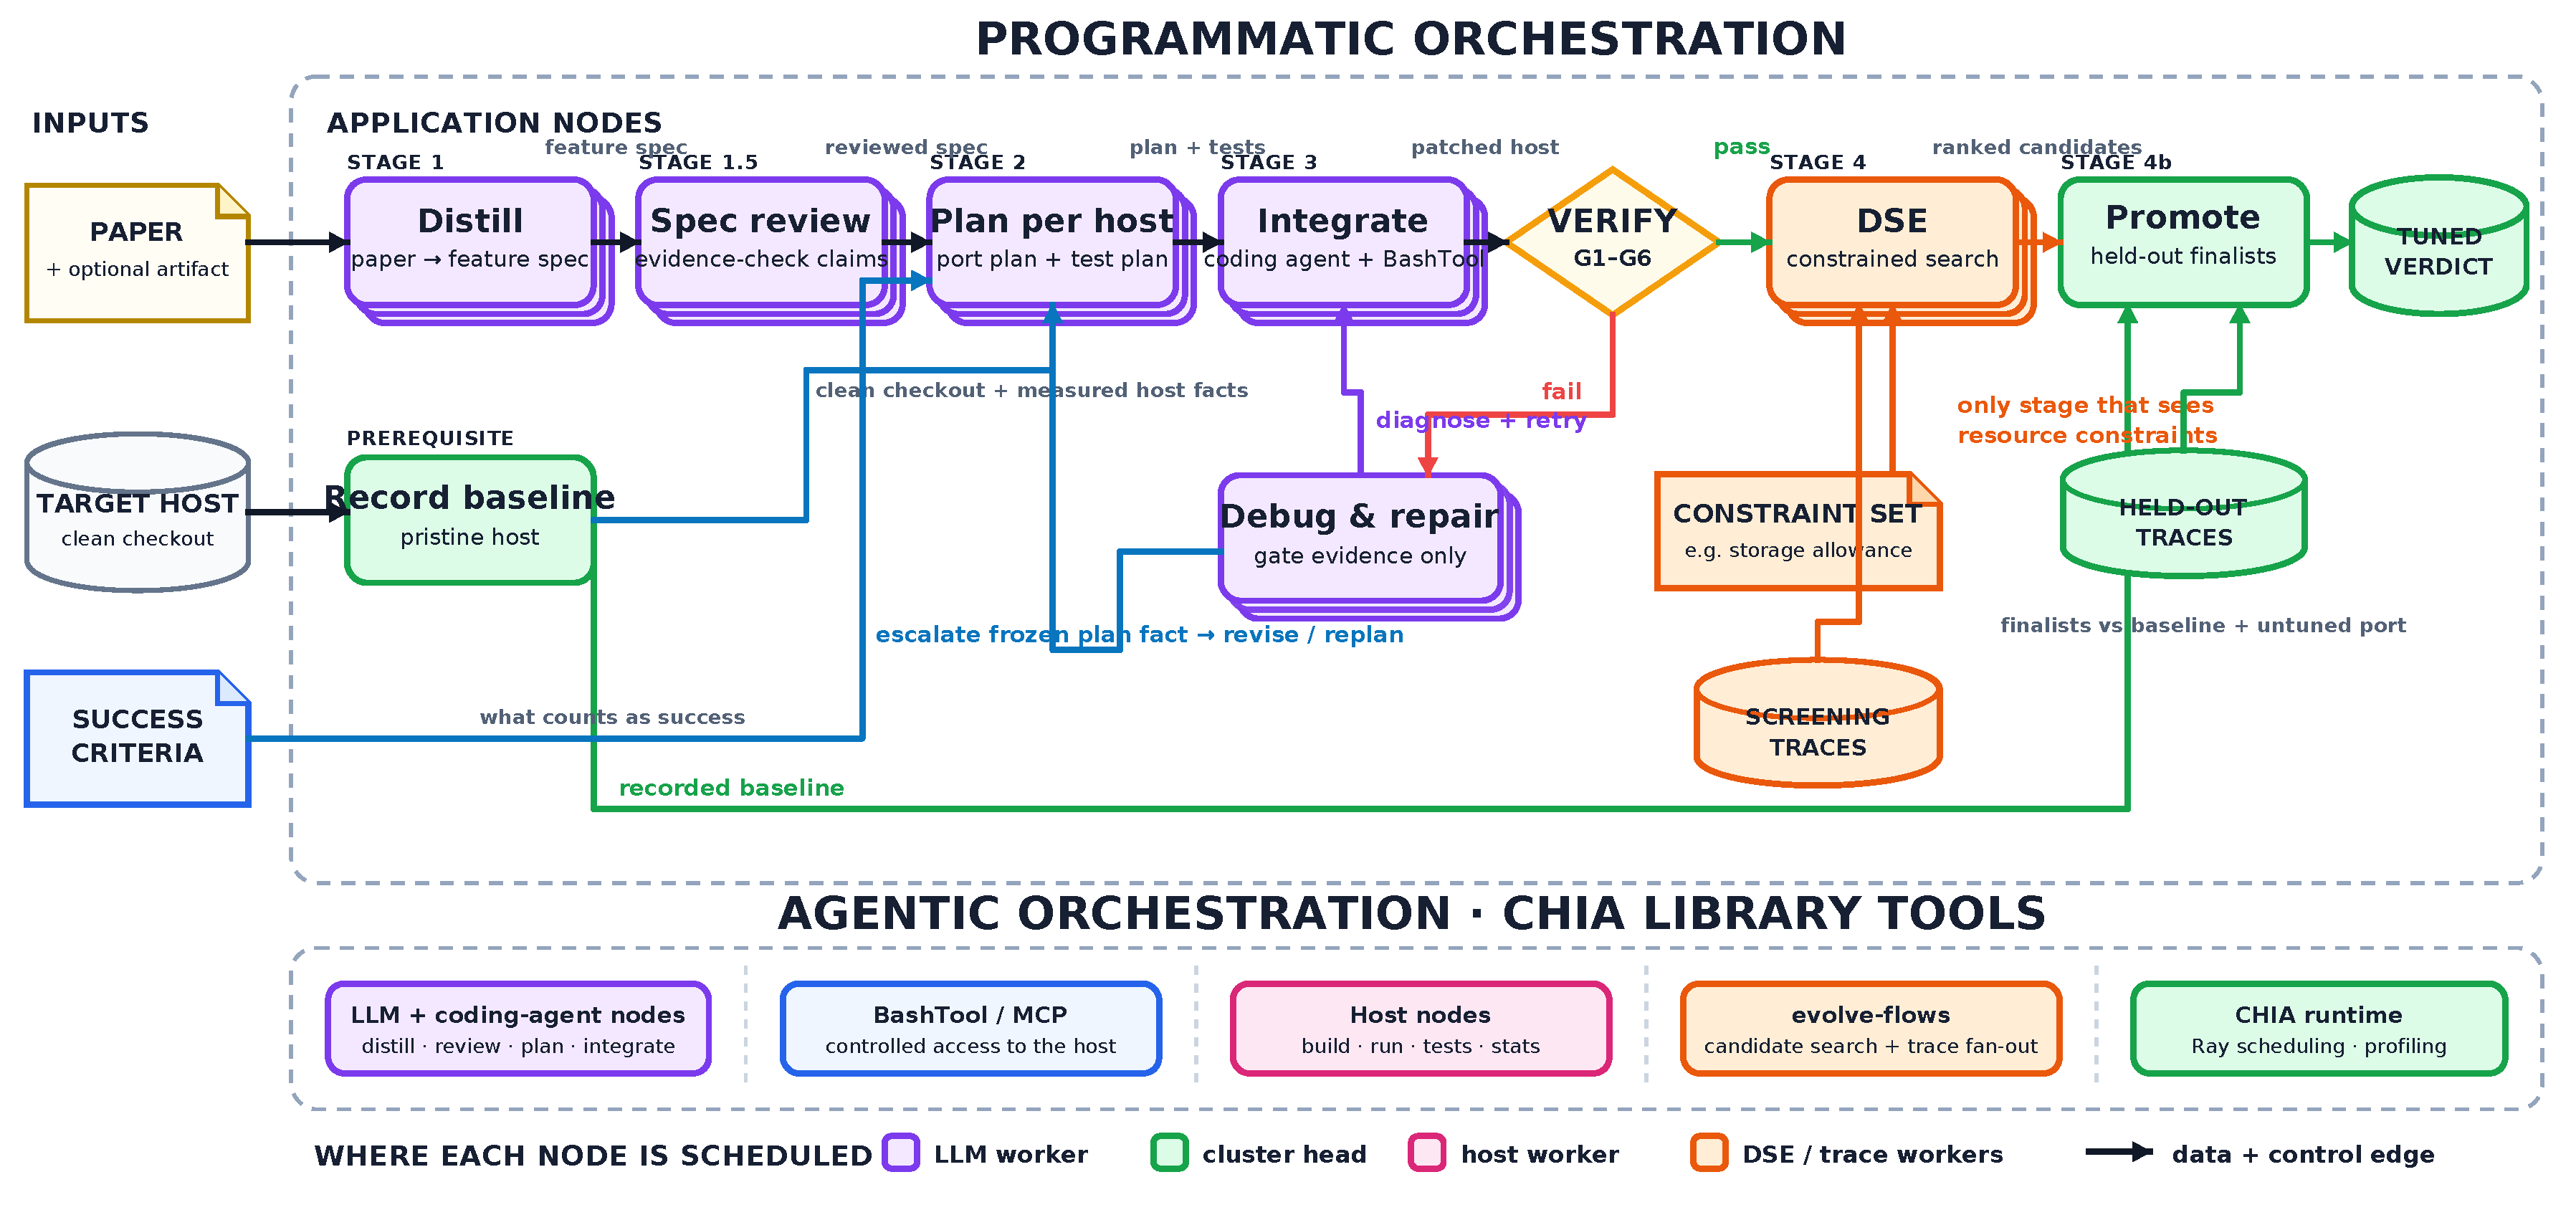
\includegraphics[width=\textwidth]{adopt-a-paper-loop}
\caption{The adopt-a-paper CHIA loop. Agentic nodes produce candidate
artifacts and edits, while programmatic edges validate specs, plans, ports and
candidates. A failed verify gate returns evidence to integration or escalates a
frozen planning fact. Only DSE receives the resource constraint, and only
held-out promotion produces the tuned-versus-baseline verdict.}
\label{fig:adopt-loop}
\end{figure*}

\begin{table}[t]
\caption{Loop stages. LLM stages are marked with $\star$.}
\label{tab:stages}
\centering
\footnotesize
\begin{tabular}{@{}p{0.2\columnwidth}p{0.35\columnwidth}p{0.33\columnwidth}@{}}
\toprule
Stage & Emits & Judged by \\
\midrule
1 Distill$^\star$ & feature spec: state, algorithms, host interfaces, knobs, size formulas, unit tests & schema, deterministic spec checks \\
1.5 Review$^\star$ & evidence-checked spec & per-claim verdict against paper text \\
2 Plan$^\star$ & port plan and test plan, host knobs, host storage formulas & coverage checks, host accounting reproduced \\
3 Integrate$^\star$ & patched host tree & gate G1--G6 \\
4 DSE$^\star$ & ranked candidate headers & constraint set, screening traces \\
Promote & verdict & held-out traces \\
\bottomrule
\end{tabular}
\end{table}

\subsection{Distill and spec review}

A distiller agent reads the paper and emits a feature spec: state elements with
sizes, algorithms as pseudocode, the host interfaces the feature needs, tunable
parameters with legal ranges, a size formula per structure, and spec-level unit
tests. The spec is the only description of $F$ that later stages read, so the
loop does not require a reference implementation.

A review stage then partitions the spec and sends each partition to a reviewer
agent. The reviewer returns a verdict per claim, quoting the paper as evidence.
Deterministic checks in code look for the defects reviewers tend to miss:
ranges that disagree with their counts, size formulas that disagree with stated
totals, and knobs that do not reach any size. We found that adding a verdict
\emph{category} matters more than sharpening prompts. Adding an
\texttt{INCONSISTENT} verdict for claims that contradict another part of the
spec cleared two errors in one review round, after six rounds across two
earlier runs had not touched them.

\subsection{Plan}

A planning agent gets a shell on a clean checkout of the host. It writes a port
plan, which says where each spec element goes and through which hook, and a
test plan with correctness tests, existing regressions and performance entries.
Because it runs the host's own tests, each existing regression carries a
measured clean-tree result. In one run it recorded the clean-tree summary
string with its trailing space intact, which showed it had run the command
rather than guessed. The plan also exposes the host's own sizing
\texttt{\#define}s as \emph{host knobs} with storage formulas. Code checks that
those formulas reproduce the host's accounting (524,615 bits on CBP2025), and
that every spec element, parameter, interface need and unit test maps to
something in the plan. A plan that fails gets one repair turn.

\subsection{Integrate and the verify gate}

A coding agent implements the plan on a copy of the host tree and runs the test
plan. The gate then judges the tree:
\begin{itemize}
\item \textbf{G1} the tree builds.
\item \textbf{G2} with the feature off, results equal the recorded baseline.
\item \textbf{G3} the spec and plan correctness tests pass.
\item \textbf{G4} with the feature on, smoke traces run clean.
\item \textbf{G5} performance entries move the ranking metric (MPKI on CBP2025)
in the claimed direction, with no regression past a band on companion metrics.
\item \textbf{G6} every storage-costing knob reaches the binary: rebuilding
with that knob at a second legal value gives a different binary.
\end{itemize}
G5 has no magnitude target. Before tuning, a port only has to move the metric
the right way; how much it moves is stage 4's question. When the gate fails,
its reasons, which include a short diagnosis (for example ``the mechanism
reaches the metric and makes it worse''), go back to the agent for another
attempt, and a plan-revision path can change hook points without re-planning
everything.

\textbf{Escalation.} The agent may not change the plan's frozen values or the
gate. If it concludes that one is wrong, it writes an escalation naming the
value by JSON pointer and giving its reason. The job then re-runs stage 2 with
the escalation attached and integrates again.

\subsection{Constraint-aware DSE and promotion}

Stage 4 mutates a generated header, \texttt{sr\_params.h}, that holds every
feature knob and host knob at the clean tree's values. We use evolve-flows'
AdaEvolve backend with Gemini models proposing edits. A constraint is
\texttt{\{metric, comparison, allowance\}}. The iso-64KiB track is the single
constraint $\texttt{storage\_bits} \le 524{,}288$. The evaluator recomputes each
candidate's storage from its header using the spec's and plan's formulas, and
refuses an over-allowance candidate before building it. Before searching, a
preflight builds each knob at a second value and stops the search if a
storage-costing knob leaves the binary unchanged, since the search would
otherwise credit bits the predictor never gave up. A candidate that compiles to
code already screened is skipped, and the evolver is told which earlier
candidate it repeated.

The search ranks on a screening list, which is small by design, so the verdict
does not come from the search. Promotion re-scores the top three candidates on
traces the search never saw, together with two references: the unmodified host
and the port at the paper's defaults. The 60-trace screening list and the
45-trace promotion list are disjoint and together cover all 105 training
traces.

%----------------------------------------------------------------------
\section{Experimental Setup}

All stages ran through \texttt{chia job submit} on a GCP cluster: one head node
and spot trace workers (\todo{final worker count and machine types; the
2026-09-23 runs used two n2-standard-2 workers with four trace slots}). The
CBP2025 kit is at commit \texttt{6074966}. Planning and integration agents use
Gemini~3.1 Pro through the Antigravity CLI. The DSE proposer uses Gemini~3.5
Flash and Gemini~3.1 Pro Preview through Vertex AI, reached through a small
OpenAI-compatible gateway that refreshes credentials, since a raw Vertex token
expires an hour into a search that runs for many hours. The inputs are the
RUNLTS paper only; we did not give the loop the RUNLTS artifact.

We report the 50th-percentile-window metrics the kit reports: MPKI
(\texttt{brmispki}) and cycles on the wrong path per kilo-instruction
(CycWPPKI). Stage 4 ranks by MPKI.

%----------------------------------------------------------------------
\section{Results}\label{sec:results}

\subsection{The gate and escalations}

The first complete integration built, matched the baseline with sR off (G2),
passed all seven spec unit tests and both existing regressions, and ran the
smoke traces clean. G5 then measured CycWPPKI rising from 388.07 to 554.61, 43
percent worse. The cause was in our host notes, not in the agent: they declared
the file holding the SC off limits. With no access to \texttt{LSUM}, the agent
built the only thing available, a standalone predictor that overrode TAGE-SC-L
whenever the two disagreed. Overriding a strong predictor with an untrained one
is expensive.

The agent did not weaken a test to get past G5. It escalated
\texttt{/host\_interfaces/4}, the plan's instruction to override the TAGE
prediction, and said why: nothing told it how confident its own sum had to be.
That is the question the SC's adaptive threshold answers. The re-plan moved the
hook into the SC's own sum. Over the first day, three escalations were raised
and all three were correct; each traced to a gap in our documentation or plan
checks, not to the agent. Two of the three classes now fail earlier, at stage 2,
through new plan checks.

Later integrations show the gate doing routine work. In one run, G5 blocked
attempts that made MPKI 87 percent worse, then exactly unchanged (the feature
was not wired to the prediction), then 1.3 percent worse. G3 blocked an attempt
whose unit tests no longer compiled, and the fifth attempt passed. In another,
the port left sR's vote out of the sum the host recomputes at update time; G5
caught that as a 0.41 percent regression.

\subsection{Search spaces that could not move}

Our first completed search could not answer the iso-budget question at all. Its
two knobs, a digest lifetime and a digest width, reached under half a percent
of sR's storage, and nothing could shrink the host to make room. We responded
in the loop rather than in the spec. The spec schema now requires size formulas
and knobs for the dimensions that set sizes (twelve knobs for sR). The plan
exposes 19 host knobs. The evaluator does storage accounting, and the preflight
checks that each knob is live.

The preflight then caught a second failure. In one port, every one of the 19
host knobs built a byte-identical binary. The agent's first turn had wired only
5 of them, and a later debugging turn restored the host file from git and
re-applied only the sR hooks. G1 to G5 cannot see this, because at default
values a wired port and an unwired one build the same binary. We added G6 to
the gate so stage 3 now fails such a port. The runs in
Table~\ref{tab:verdict} labelled ``hand-wired'' used that port after we wired
the 19 host knobs by hand, without re-running stage 3 under G6. They show how
sR tunes on this port. They do not show that stage 3 produces a tunable port
unaided.

We also discarded our 192~KiB runs as a verdict. The kit's default host is
64~KB-class, so at 192~KiB the search simply bought host capacity the baseline
never had: the best candidate doubled the TAGE tables and left sR alone.

\subsection{The iso-64KiB verdict}

At 64~KiB the host is already over the allowance, so any candidate that
includes sR must shrink the host to pay for it. Table~\ref{tab:verdict} gives
three searches. R1 used a fully loop-produced port, a short search (24
iterations on 8 screening traces), and 16 held-out traces. R2 and R3 used the
hand-wired port, 77 to 79 iterations on the 60-trace screening list, and the 45
remaining traces. They differ in whether sR's in-flight checkpoint state
(16,640 bits, used to restore the register table after a misprediction) is
charged to the budget.

\begin{table}[t]
\caption{Iso-64KiB verdicts on held-out traces. Change is relative to the
unmodified host (lower is better).}
\label{tab:verdict}
\centering
\footnotesize
\begin{tabular}{@{}llrrr@{}}
\toprule
Run & Variant & Bits & MPKI & CycWPPKI \\
\midrule
R1: loop port, & host alone & 524,615 & --- & --- \\
\quad 16 traces & sR defaults (over budget) & 578,478 & $-0.63\%$ & $-0.03\%$ \\
 & tuned & 524,206 & $+0.76\%$ & $+0.81\%$ \\
\midrule
R2: hand-wired, & host alone & 524,615 & --- & --- \\
\quad state charged, & sR defaults (over budget) & 595,118 & $-0.17\%$ & $+0.15\%$ \\
\quad 45 traces & tuned & 523,918 & $\mathbf{-0.34\%}$ & $+0.07\%$ \\
\midrule
R3: hand-wired, & tuned & 524,254 & $+0.75\%$ & $+0.69\%$ \\
\quad state exempt, 45 &  &  &  &  \\
\bottomrule
\end{tabular}
\end{table}

Only R2's tuned candidate beats the host on held-out MPKI, by 0.34 percent,
and it is slightly worse on CycWPPKI. It lowers MPKI on 23 of the 45 traces and
raises it on 22. Combining its held-out result with its in-sample screening
result gives $-0.31$ percent MPKI and $+0.13$ percent CycWPPKI over all 105
traces; the 60-trace half is not independent evidence, since the candidate was
selected there. The winner cut the tagged banks (low 10 to 8, high 20 to 15)
and halved one sR weight table, and spent the savings on wider TAGE tags, wider
SC weights, more bimodal hysteresis and a larger sR usefulness table. The
proposer's own comment in that header misdescribes several of these changes, a
reminder that the evaluator, not the proposer, has to be the source of truth.

The negative results are consistent. sR at the paper's defaults on the full
host lowers MPKI in every run (0.17 to 0.63 percent), but it does not fit.
Every candidate that fits pays for sR by removing TAGE capacity, and on most
trace mixes that costs more than sR returns. R3 is the clearest case: it had
16,640 more bits to spend than R2, yet its best screening candidate never beat
the host even in-sample, and its screening winner did not stay the winner on
held-out traces. R2 and R3 differ by more than their constraint does, so
search variance is at least as large as the effects being measured.

The per-trace picture explains why screening lists matter. In R1, sR at its
defaults improved compress traces by about 8 percent and fp by 0.6 to 1.4
percent, while most int and web traces got 0.4 to 2.5 percent worse. R1's
8-trace screening list had no compress trace, so the search never saw the
family where sR helps most.

We cannot yet say what fraction of sR's gain the tuned port recovers. That
needs sR's contribution inside RUNLTS, from an sR-off ablation of the
artifact, which we have not run.

\subsection{A second host}

The loop has no per-host branches; a host is an adapter. We brought up gem5
v25.1~\cite{gem5} with its TAGE-SC-L 64~KB predictor on an O3 ARM CPU and 28
workloads. The build, fan-out, baseline and gate all work, and gem5 runs are
bit-for-bit repeatable, which G2 relies on. Stage 2 produced an accepted gem5
plan after one repair turn. Stage 3 has not yet passed: across two runs and six
attempts, G5 measured conditional MPKI 7.4 to 9.5 percent worse and IPC 1.8 to
2.3 percent worse, and the last attempt did not build. The gate blocked every
one. \todo{update if a gem5 port passes before submission.}

%----------------------------------------------------------------------
\section{Discussion}

\textbf{Deterministic gates carry the loop.} Every broken port we saw was
caught by plain code, and several broke in ways an agent reviewing its own
work would plausibly miss: a port correct on every unit test but 43 percent
worse, a port whose knobs were silently disconnected, a port whose feature never
reached the prediction. The gate's diagnostic text was often what let the next
attempt succeed.

\textbf{Failures cluster at hand-offs.} The failures that cost us most were not
coding errors inside a stage. They were facts lost between stages: a host note
that was wrong, a spec with knobs that could not change a size, a plan whose
host knobs a later debugging turn quietly un-wired. Each was fixed by adding a
mechanism (a plan check, a schema field, a gate condition) rather than by
correcting the artifact, so the next run is evidence about the loop.

\textbf{Mechanisms beat prompt tuning.} Adding a missing verdict category, a
missing gate condition, or a missing check resolved problems at once.
Sharpening a heuristic in a prompt was open-ended and often did not converge.

\textbf{Tuning is where the verdict lives, and it is noisy.} Without DSE, sR
looks like a small win (it lowers MPKI at the paper's defaults). At fixed
storage the answer is ``roughly break-even, depending on the search.'' An
untuned comparison would have given the wrong impression. But three searches
disagree in sign, so a single search is not a verdict either. Repeated
searches, or a longer one, are needed before the verdict is stable.

\subsection{Threats to validity}
\begin{itemize}
\item R2 and R3 used a port whose host knobs were wired by hand (above).
\item After the first escalation, we corrected the host notes that planning and
integration agents read. As written, that correction also states how sR should
enter the SC sum, which is a feature-specific answer rather than a host fact.
Later ports therefore did not answer that question unaided.
\todo{re-run with feature-neutral host notes, or state this more prominently.}
\item The port hard-codes sR's $\times 2.5$ usefulness multiplier, so that
dimension was never searched.
\item The iso-64KiB baseline is 327 bits over the allowance, so every feasible
candidate uses slightly less storage than the baseline.
\item G2 proves feature-off equivalence on sample traces, not on the
performance traces.
\end{itemize}

%----------------------------------------------------------------------
\section{Related Work}

AlphaEvolve~\cite{alphaevolve} and its open implementations use LLMs as mutation
operators in an evolutionary search over programs; our stage 4 is an instance,
with the program restricted to a header of knob values and a hard constraint
checked before evaluation. CHIA~\cite{chia} provides agentic loops for
hardware, including gem5 alignment and evolutionary discovery case studies; our
loop turns those patterns into a reusable ``adopt a paper'' capability.
Championship simulators such as CBP2025~\cite{cbp2025kit} and
ChampSim~\cite{champsim} fix a storage budget so that predictors can be
compared fairly; we move that idea from the contest into the evaluation of a
single feature. \todo{add LLM-for-architecture and LLM-for-RTL related work.}

%----------------------------------------------------------------------
\section{Conclusion and Future Work}

We built a loop that ports a published feature from its paper into a real
simulator, verifies it with deterministic gates, and tunes it jointly with the
host under a storage constraint. On sR in CBP2025 TAGE-SC-L at 64~KiB, the
loop's verdict is that sR roughly pays for itself and no more. Its benefit at
the paper's defaults is real but smaller than the TAGE capacity it displaces,
and the tuned margin is within the variance between searches.

Next steps: re-integrate under G6 so the tuned port is fully loop-produced;
screen on a list that includes every workload family; run repeated searches to
put error bars on the verdict; measure sR's gain inside the RUNLTS artifact to
anchor the recovery target; finish the gem5 and ChampSim ports; run the
paper-only versus paper-plus-artifact ablation; and report token and compute
cost per accepted change from CHIA's profiler. \todo{cost numbers.}

\section*{Acknowledgment}
This work was done for the Agentic Approaches to Architecture CHIA Hackathon.
\todo{credit and funding.}

\begin{thebibliography}{00}
\bibitem{runlts} T. Koizumi, T. Maekawa, M. Mizuno, M. Kuroki, T. Tsumura, and
R. Shioya, ``RUNLTS: Register-value-aware predictor utilizing nested large
tables,'' in \emph{Championship Branch Prediction (CBP2025), held with ISCA
2025}, Tokyo, Japan, Jun. 2025, pp. 1--6.
\bibitem{tagescl} A. Seznec, ``TAGE-SC-L branch predictors again,'' in
\emph{5th JILP Workshop on Computer Architecture Competitions (JWAC-5):
Championship Branch Prediction (CBP-5)}, 2016.
\bibitem{cbp2025kit} CBP2025 simulation framework.
\url{https://github.com/ramisheikh/cbp2025}
\bibitem{chia} CHIA. \url{https://github.com/ucb-bar/chia}
\bibitem{evolveflows} evolve-flows. \url{https://github.com/ucb-bar/evolve-flows}
\bibitem{alphaevolve} A. Novikov \emph{et al.}, ``AlphaEvolve: A coding agent
for scientific and algorithmic discovery,'' 2025. \todo{check citation}
\bibitem{gem5} J. Lowe-Power \emph{et al.}, ``The gem5 simulator: Version
20.0+,'' arXiv:2007.03152, 2020.
\bibitem{champsim} N. Gober \emph{et al.}, ``The Championship Simulator:
Architectural simulation for education and competition,'' arXiv:2210.14324,
2022.
\end{thebibliography}

\end{document}
